
%%%%%%%%%%%%%%%%%%%%%%% file typeinst.tex %%%%%%%%%%%%%%%%%%%%%%%%%
%
% Author: Mauricio Matamoros
% Updated: July 3, 2017
% Contact: mauricio@robocupathome.org
%
% This is the LaTeX source for the TDPTemplate using
% the LaTeX document class 'llncs.cls' Springer LNAI format
% used in the RoboCup Symposium submissions.
% http://www.springer.com/computer/lncs?SGWID=0-164-6-793341-0
%
% It may be used as a template for your own TDP - copy it
% to a new file with a new name and use it as the basis
% for your Team Description Paper
%
% NB: the document class 'llncs' has its own and detailed documentation, see
% ftp://ftp.springer.de/data/pubftp/pub/tex/latex/llncs/latex2e/llncsdoc.pdf
%
% Remark: Last page with specs won't be included in Camera ready TDP's.
%
%%%%%%%%%%%%%%%%%%%%%%%%%%%%%%%%%%%%%%%%%%%%%%%%%%%%%%%%%%%%%%%%%%%

\documentclass[runningheads,a4paper]{llncs}
\usepackage{amssymb}
\setcounter{tocdepth}{3}
\usepackage{graphicx}
\usepackage{amssymb}
\usepackage[utf8]{inputenc}
\usepackage{url}
\usepackage{float}
\usepackage{amsmath}
\usepackage{graphicx}
\usepackage{wrapfig}
\usepackage{fancyhdr}
\usepackage{titling}
\usepackage{lipsum}
\newcommand{\robospecs}{%
	\newpage%
	\pagenumbering{gobble}%
	\pagestyle{fancy}%
	\fancyhf{}%
	\chead{$|$}
	\rhead{\footnotesize\thetitle}%
	\lhead{\footnotesize\theauthor}%
	\rfoot{Robot software and hardware specification sheet}%
}

\newcommand{\BnL}[1][1em]{ 
\includegraphics[width=#1]{images/bnl.jpg} }


%%%%%%%%%%%%%%%%%%%%%%%%%%%%%%%%%%%%%%%%%%%%%%%%%%%%%%%%%%%%%%%%%%%%%%%%%%%%%%%%%%%%
%
% Title
%
%%%%%%%%%%%%%%%%%%%%%%%%%%%%%%%%%%%%%%%%%%%%%%%%%%%%%%%%%%%%%%%%%%%%%%%%%%%%%%%%%%%%
\title{Lipsum 2018 Team Description Paper}

\author{Main-author \and Co-author \and Team Members}
\institute{Affiliation name and address, \\
\texttt{http://devoted-web-site.url}}


\begin{document}
\maketitle

%%%%%%%%%%%%%%%%%%%%%%%%%%%%%%%%%%%%%%%%%%%%%%%%%%%%%%%%%%%%%%%%%%%%%%%%%%%%%%%%%%%%
%
% Abstract
%
%%%%%%%%%%%%%%%%%%%%%%%%%%%%%%%%%%%%%%%%%%%%%%%%%%%%%%%%%%%%%%%%%%%%%%%%%%%%%%%%%%%%

\begin{abstract}

In your abstract, please state your main research line and your achievements of this year (on which problem or set of problems are you focusing all the team efforts). Tell why this research is important, how are you approaching to the problem solution and which results do you expect to obtain.

\end{abstract}


%%%%%%%%%%%%%%%%%%%%%%%%%%%%%%%%%%%%%%%%%%%%%%%%%%%%%%%%%%%%%%%%%%%%%%%%%%%%%%%%%%%%

\section{Introduction}
While writing the TDP, focus on your current research, clearly stating all scientific contribution, and why are they important for you and the league. The length of the TDP is limited to 6 pages. Please notice that changes to the margins, space between paragraphs, and font size are not allowed (such TDP will be rejected). We suggest to leave the hardware and software description for the end of the paper.

Remember that the TDP must contain the following information:

\begin{itemize}
	\item Description of the hardware and software including a list of integrated externally available components (including commercial products, freeware, Open Source, etc.)
	\item Innovative technology and scientific contribution
	\item Photo(s) of the robot
	\item Focus of research/research interests
	\item Re-usability of the system for other research groups
	\item Applicability of the robot in the real world
\end{itemize}

\section{Background}
% We are Buy n Large. We have no competitors so no background is required.
\lipsum[1-3]

\section{BnL Trash Seeker Algorithm (Main research)}
\lipsum[4-14]

\section{BnL All-purpose Speech Recognizer (Main research)}
\lipsum[15-20]

\section{Other relevant contributions}
\lipsum[21]
\subsection{Dirt Detector Algorithm}
\lipsum[22-25]
\subsection{Green Plant Seeker Algorithm}
\lipsum[25-29]
\subsection{Trash Seeker Algorithm}
\lipsum[30-34]

\section{Experiments and results}
\lipsum[35-39]

\section{Conclusions and future work}
\lipsum[40-43]

%%%%%%%%%%%%%%%%%%%%%%%%%%%%%%%%%%%%%%%%%%%%%%%%%%%%%%%%%%%%%%%%%%%%%%%%%%%%%%%%%%%%
%
% Bibliography
%
%%%%%%%%%%%%%%%%%%%%%%%%%%%%%%%%%%%%%%%%%%%%%%%%%%%%%%%%%%%%%%%%%%%%%%%%%%%%%%%%%%%%

\section*{Bibliography}
\bibliographystyle{unsrt}
\bibliography{bibliography}

%%%%%%%%%%%%%%%%%%%%%%%%%%%%%%%%%%%%%%%%%%%%%%%%%%%%%%%%%%%%%%%%%%%%%%%%%%%%%%%%%%%%
%
% Robot Specifications
%
%%%%%%%%%%%%%%%%%%%%%%%%%%%%%%%%%%%%%%%%%%%%%%%%%%%%%%%%%%%%%%%%%%%%%%%%%%%%%%%%%%%%

\robospecs
\section*{EVA Software and External Devices [DSPL Template]}
% In this section briefly describe the software and hardware of the robot

\setlength\intextsep{0pt}
\begin{wrapfigure}[10]{r}{0.3\textwidth}
	\centering
	
\includegraphics[width=0.4\textwidth]{images/eva.png}
	\caption{Robot EVA}
	\label{fig:eva}
\end{wrapfigure}

We use a standard EVA robot from \textit{Buy'N Large}. No modifications have been applied.

\section*{Robot's Software Description}
% Please describe in this section the software you are using to control your robot. Consider the following example:

\textit{For our robot we are using the following software:}

\begin{itemize}
	\item Platform: \BnL Operating System
	\item Face recognition: None. Not designed for human interaction.
	\item Object recognition: \BnL Green Plant Seeker Algorithm (See previous sections).
	\item Arms control and two-hand coordination: \BnL automatic controller \cite{bnl2}.
\end{itemize}

\section*{External Devices}
% Please describe in this section the external devices used by your robot. Consider the following example:

\textit{EVA robot relies on the following external hardware:}

\begin{itemize}
	\item \BnL Mother-ship
	\item \BnL Data Cluster
	\item $3 \times$ \BnL Ultra-Power laptops.
\end{itemize}

\section*{Cloud Services}
% Please describe in this section the Cloud Services and online software used by your robot. Consider the following example:

\textit{EVA connects the following cloud services:}
\begin{itemize}
	\item Localization and mapping: \BnL Geolocalization system \cite{bnl3}.
	\item Navigation: \BnL Navigator
	\item Speech recognition: \BnL All-purpose recognizer \cite{bnl1}.
	\item Speech generation: \BnL Speech synthesizer.
\end{itemize}

\newpage
\section*{Robot WALL-E Hardware Description [OPL Template]}
% In this section briefly describe the software and hardware of the robot

\setlength\intextsep{0pt}
\begin{wrapfigure}[10]{r}{0.3\textwidth}
	\centering
	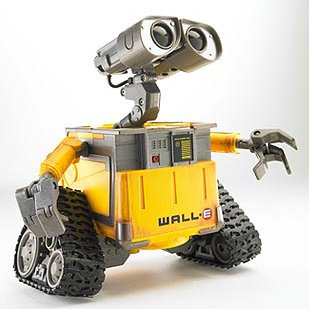
\includegraphics[width=0.4\textwidth]{images/wall-e.jpg}
	\caption{Robot WALL-E}
	\label{fig:wall-e}
\end{wrapfigure}

Robot WALL-E has the patented \textit{\BnL Optimized Design} for garbage recollection. Specifications are as follows:

\begin{itemize}
	\item Base: \BnL all-terrain base (differential pair), 2.5m/s max speed.
	\item Torso: \BnL compressor with solar charger.
	\item Left and right arms: Mounted on torso. \BnL 7DOF, anthropomorphic. Maximum load: 20kg.
	\item Neck: \BnL telescopic neck with pan and tilt.
	\item Head: 3DOF \BnL Expressive Eyes
	\item Robot dimensions: height: 1.2m (max), width: 0.7m depth 0.8m
	\item Robot weight: 50kg.
\end{itemize}

\noindent\textit{Also our robot incorporates the following devices:}

\begin{itemize}
	\item \BnL Battery charge indicator
	\item \BnL Auto-focus all-purpose cameras
	\item \BnL 7DOF heavy duty fingers
	\item \BnL Cockroach
\end{itemize}

\section*{Robot's Software Description}
% Please describe in this section the software you are using to control your robot. Consider the following example:

\textit{For our robot we are using the following software:}

\begin{itemize}
	\item Platform: \BnL Operating System
	\item Navigation: \BnL Navigator
	\item Face recognition: None. Not designed for human interaction.
	\item Speech recognition: \BnL All-purpose recognizer \cite{bnl1}.
	\item Speech generation: None. Not designed for human interaction.
	\item Object recognition: \BnL Trash Seeker Algorithm (See previous sections).
	\item Arms control and two-hand coordination: \BnL automatic controller \cite{bnl2}.
\end{itemize}

\section*{External Devices}
% Please describe in this section the external devices used by your robot. Consider the following example:

\textit{WALL-E robot relies on the following external hardware:}

\begin{itemize}
	\item \BnL Garbage Compactor
	\item \BnL EVA unit
	\item \BnL Data Cluster
	\item $3 \times$ \BnL Ultra-Power laptops.
\end{itemize}

\section*{Cloud Services}
% Please describe in this section the Cloud Services and online software used by your robot. Consider the following example:

\textit{WALL-E connects the following cloud services:}
\begin{itemize}
	\item Localization and mapping: \BnL Geolocalization system \cite{bnl3}.
\end{itemize}
\newpage
\section*{M-O Software and External Devices [SSPL Template]}
% In this section briefly describe the software and hardware of the robot

\setlength\intextsep{0pt}
\begin{wrapfigure}[10]{r}{0.3\textwidth}
	\centering
	
\includegraphics[width=0.4\textwidth]{images/m-o.png}
	\caption{Robot M-O}
	\label{fig:m-o}
\end{wrapfigure}

We use a standard \textit{Buy'N Large} M-O robot unit. To differntiate our unit, an orange marker has been added on its top.

\section*{Robot's Software Description}
% Please describe in this section the software you are using to control your robot. Consider the following example:

\textit{For our robot we are using the following software:}

\begin{itemize}
	\item Platform: \BnL Operating System
	\item Face recognition: None. Not designed for human interaction.
	\item Speech generation: None. Not designed for human interaction.
	\item Object recognition: \BnL Dirt Detector Algorithm (See previous sections).
	\item Mop unit: \BnL automatic controller \cite{bnl2}.
\end{itemize}

\section*{External Devices}
% Please describe in this section the external devices used by your robot. Consider the following example:

\textit{M-O robot relies on the following external hardware:}

\begin{itemize}
	\item \BnL Mother-ship
	\item \BnL Data Cluster
	\item $3 \times$ \BnL Ultra-Power laptops.
\end{itemize}

\section*{Cloud Services}
% Please describe in this section the Cloud Services and online software used by your robot. Consider the following example:

\textit{M-O connects the following cloud services:}
\begin{itemize}
	\item Localization and mapping: \BnL Geolocalization system \cite{bnl3}.
	\item Navigation: \BnL Navigator
	\item Speech recognition: \BnL All-purpose recognizer \cite{bnl1}.
\end{itemize}

\nocite{*}

\end{document} 
